\documentclass[a4paper, 12pt, oneside]{article}

\setlength{\parindent}{0cm}
\setlength{\parskip}{0cm}

\usepackage[english,russian]{babel}
\usepackage{titlesec}
\usepackage[T2A]{fontenc}
\usepackage[utf8]{inputenc}
\usepackage{ragged2e}
\usepackage{hyperref}
\usepackage{standalone}
\usepackage{minted}
\setmintedinline{frame=lines, framesep=2mm, baselinestretch=1.5, bgcolor=LightGray, breaklines,fontsize=\scriptsize}
\setminted{frame=lines, framesep=2mm, baselinestretch=1.5, bgcolor=LightGray, breaklines,fontsize=\scriptsize}
\usepackage{xcolor}
\definecolor{LightGray}{gray}{0.9}
\usepackage{graphicx}
\usepackage{adjustbox}
\usepackage[left=3cm,right=1.5cm,
    top=2cm,bottom=2cm,bindingoffset=0cm]{geometry}
\usepackage{ upgreek }
\usepackage[shortlabels]{enumitem}
\usepackage{multirow}
\usepackage{amsmath}
\usepackage{amssymb}
\usepackage{pifont}
\usepackage{titlesec}
\usepackage{longtable}

\usepackage{pgfplots}
\usepackage{verbatim}
\usetikzlibrary{positioning}
\usetikzlibrary{shapes.geometric}
\usetikzlibrary{shapes.misc}
\usetikzlibrary{calc}
\usetikzlibrary{chains}
\usetikzlibrary{matrix}
\usetikzlibrary{decorations.text}
\usepackage{fontspec}
\usepackage{booktabs}
\usetikzlibrary{backgrounds}
\usepackage{capt-of}
\usepackage{caption} %заголовки плавающих объектов

\captionsetup[figure]{name=Рисунок}

\newcounter{labeltablecounter}
\renewcommand{\thelabeltablecounter}{
    \arabic{labeltablecounter}
}

\DeclareCaptionFormat{tablecaption}
{
    \begin{flushright}
        \textit{#1}
    \end{flushright}
    \begin{center}
        \textbf{#3}
    \end{center}
}

\DeclareCaptionFormat{imagecaption}
{%
    #1#2#3
}

\renewcommand{\baselinestretch}{1.5}

\graphicspath{ {./images/} }
\makeatletter
\AddEnumerateCounter{\asbuk}{\russian@alph}{щ}
\makeatother
\setmonofont{Consolas}
\setmainfont{Times New Roman}

\newcommand\textbox[1]{
    \parbox{.45\textwidth}{#1}
}

\newcommand\makenewfig[3] {
    \captionsetup{format=imagecaption}
    \begin{center}
        #1
        \nopagebreak
        \captionof{figure}{#2}
        \nopagebreak
        \label{#3}
    \end{center}
}

\newcommand\labeltable[3] {
    \captionsetup{format=tablecaption}
    \begin{table}[H]
        \caption{#2}
        \begin{center}
            #1
        \end{center}
        \label{#3}
    \end{table}
}

\titleformat*{\section}{\Large\bfseries}
\titleformat*{\subsection}{\large\bfseries}
\newcommand{\anonsection}[1]{\section*{#1}\addcontentsline{toc}{section}{#1}}

\newcommand{\specialcell}[2][c]{%
    \begin{tabular}[#1]{@{}c@{}}
        #2
    \end{tabular}}

\begin{document}
    \linespread{1.5}
    \setlength{\parskip}{0cm}

    \pagenumbering{gobble}

    \justifying
    \begin{center}
        \small{
            МИНИCТЕРCТВО НАУКИ И ВЫCШЕГО ОБРАЗОВАНИЯ \\РОCCИЙCКОЙ ФЕДЕРАЦИИ
            \bigbreak
            ФЕДЕРАЛЬНОЕ ГОCУДАРCТВЕННОЕ БЮДЖЕТНОЕ ОБРАЗОВАТЕЛЬНОЕ УЧРЕЖДЕНИЕ ВЫCШЕГО ОБРАЗОВАНИЯ \\
            \bigbreak
            \textbf{«БЕЛГОРОДCКИЙ ГОCУДАРCТВЕННЫЙ \\ТЕХНОЛОГИЧЕCКИЙ УНИВЕРCИТЕТ им. В. Г. ШУХОВА»\\ (БГТУ им. В.Г. Шухова)} \\
            \bigbreak
            Кафедра программного обеспечения вычислительной техники и автоматизированных систем\\}
    \end{center}

    \vfill
    \begin{center}
        \large{
            \textbf{
                Отчёт по производстввенной преддипломной практике}}\\
    \end{center}
    \vfill
    \hfill\textbox{
        Выполнил: ст. группы ПВ-223\\Пахомов Владислав Андреевич\\
        \_\_\_\_\_\_\_\_\_\_\_\_\_\_\_\_\_\_\\
        (подпись студента)
        \bigbreak
        Проверил: Картамышев Сергей Владимирович
        \_\_\_\_\_\_\_\_\_\_\_\_\_\_\_\_\_\_\\
        (подпись руководителя практики)
        \bigbreak
        Оценка \_\_\_\_\_\_\_\_\_\_\_\_\_\_\_\_\_\_
    }
    \vfill\begin{center}
              Белгород 2026 г.
    \end{center}
    \newpage
    \renewcommand{\contentsname}{Оглавление}
    \tableofcontents\newpage
    
\section{ВВЕДЕНИЕ}

Мир современного человека всё больше переходит в цифровое пространство, и это не удивительно.
Цифровое пространство обладает неоспоримыми преимуществами при работе с информацией:

\begin{itemize}[label=$\bullet$]
	\item Дешёвое хранение информации, а значит её большой объём
	\item Большая скорость передачи информации
	\item Возможность обрабатывать большое количество информации очень быстро
	\item Качество хранимой информации
\end{itemize}

Эти факторы так или иначе и стали решающими
в решении хранения данных как в быту человека, так и в бизнес-процессах и в творчестве.

Самым ярким и приближённым к цифровому пространству примером является профессия программиста.
На это влияет как сама специфика и предназначение профессии, так и вышеописанные процессы.
Можно ли себе представить программиста, который совсем не владеет компьютером? 
Конечно же нет. Возьмут ли на работу программиста, который продолжает хранить весь свой 
код на листах бумаги? Только если эта компания почему-то любит запускать очень старые ракеты. 
Современного конкурентноспособного разработчика сложно представить без умных текстовых редакторов, 
хранения кода в облаке, автоматизации процессов доставки клиентам, нейронных сетей помогающих 
в написании кода (а иногда ещё и пишущих за них).

Сама профессия по личному мнению автора лежит на стыке творческого процесса и бизнес процессов 
в разной степени важности в зависимости от разрабатываемого продукта.
Она требует как изобретательности, креативности и нестандартных подходов при решении различных задач, 
так и соответствия конкретным рамкам, условиям и отлаженным процессам. 

На примере профессии программиста можно увидеть, насколько сильно может интегрироваться цифровое 
пространство в сферу требующую как творческого подхода, так и точности,
и насколько много пользы оно может принести при решении задач. Важно, однако, отметить, что
цифровое пространство всё ещё не может полностью вытеснить другие подходы. Это такой же инструмент, 
как, например, молоток. Оно решает конкретные проблемы, связанные преимущественно с информацией.

Одна из сфер, которая очень похожа на программирование, является музыкальная сфера. 
Она также требует творческого подхода, но также задаёт в себе определённые рамки.

И да, за последнее время интеграция цифрового пространства в этой сфере тоже сильно продвинулась. 
Сервисы музыкального стриминга, согласно исследованиям, используют уже более трети 
россиян, а рост аудитории продолжается. В процессе написания музыки всё чаще используются 
DAW, умеющие работать с продвинутым оборудованием записи; синтез звука и его обработка тоже проходили 
очень долгий путь эволюции. 

Однако на рынке продюссирования музыки почему-то очень мало инструментов, которые помогают 
в разработке аудиоданных. Множество продюссеров всё ещё складывают свои проекты в крайне неорганизованное
хранилище часто представляющее собой обычную папку на локальных персональных компьютерах. А 
если данные будут утеряны, то обычно с этим ничего поделать нельзя и их приходится восстанавливать
"по памяти".

И такие проблемы очень легко решить. Тем более, для них уже есть решение. И их можно 
позаимствовать из той же ранее расмотренной профессии программиста. Облачное хранилище данных
позволит избежать проблемы утери данных а также позволит делиться ими касанием пальца, что 
тоже повысит эффективность общения с коллегами. Хранение предыдущих версий позволит 
возвращаться к старым концепциям, пересматривать их, рефлексировать и адаптировать в разработке.
Распространение данных в централизованной платформе гораздо более удобно для конечного потребителя
в лице дистрибьютора или слушателя. Дополнение платформы в виде бизнес-сущностей позволит 
дистрибьюторам при публикации полученных композиций.

Создание единой платформы также создаёт множество задач по обработке и выдаче данных. 
Аудиоданные могут быть очень большими, особенно если это демонстрационные записи, не отличающиеся
особой лаконичностью. В связи с этим должна быть также возможность порционной выдачи данных в реальном 
времени.

Первая глава посвящена анализу предметной области, в ней рассматривается актуальность создания 
сервиса, выполняется сравнительный анализ готовых решений, формируются функицональные и нефункциональные
требования к разрабатываемому сервису.

Вторая глава описывает проектирование: общие архитектурные паттерны, рассмотрена клиент-сверверная
составляющая и интерфейсы их взаимодействия, архитектура хранилищей данных

Третья глава содержит структуру программного обеспечения: модели и сервисы, конкретные библиотеки при 
реализации.

Четвёртая глава описывает инфраструктуру сервиса: процессы контейнеризации, выдачи статических данных, 
конфигурации Nginx и обратного проксирования, подключения графических устройств для работы 
алгоритма сжатия.

Разрабатываемый сервис соответствует концепциям и тенденциям развития отрасли, поддерживаемый 
и расширяемый. Цель реализуемого сервиса - управление процессами разработки 
композиции а также упрощение её распространения в профессиональной среде.

\section{ОБЗОР ПРЕДМЕТНОЙ ОБЛАСТИ}
\subsection{Актуальность разрабатываемого сервиса}

Разработка музыкальный композиций занимает одно из важных мест на сегодняшнем рынке. Количество
потребителей музыкального контента каждый день продолжает расти, о чём говорит статистика
музыкальных стриминговых сервисов. Однако инструментов
для управления разработки и обеспечения её эффективности у современных продюссеров представлено очень мало.

На текущий момент самым распространённым способом хранения аудиоданных является их хранение на локальных
носителях или же на хранителе персональных компьютеров. Повреждение или утеря хранилищ приведёт к
утере данных а также к необходимости их восстановления с нуля, что будет занимать
очень много времени а также имеет риск привести к невозможности восстановления изначального варианта ввиду
несовершенства человеческой памяти.

Важным аспектом является развитие композиции. Один проект или же композиция могут иметь несколько 
различных форм. Например, может измениться инструментальная или вокальная партия. Кроме того, отслеживание предыдущих
версий позволит найти более удачный вариант исполнения и использовать наработки в новой итерации. Также вид композиции 
может сильно разниться в зависимости от его целей и вариантов исполнений. В отношении живой музыки это может быть
композиция записанная в живом исполнении или в студии. Путём введения запрета на редактирование и удаление данных
можно обеспечить как улучшенные гарантии хранения данных, так и сохранение всех версий композиции.

Для возможности отделения музыкальных композиций по их назначению можно ввести понятие тегов. Тег - короткое 
строковое описание версии, которое описывает цель этого релиза.

При условии наличия большого количества версий композиции возникает вопрос составления серий композиций, или же плейлистов. 
Так как каждый из треков имеет свою определённую ценность и форму, плейлист так же может иметь свою ценность. 
Например, владельцу площадки для выступлений будет не очень интересно услышать, как группа будет звучать в живой записи, гораздо большую ценность
для него будет предоставлять живое выступление. Плейлисты позволят быть гораздо более гибким и предоставлять
различным заказчикам интересную для его задач информацию.

Предоставление служебной информации также сильно облегчит процесс взаимодействия с проектом. 
В любой момент можно посмотреть название проекта, исполнителей, описание без дополнительного обращения, что 
позволит увеличить эффективность разработки. 

Важным аспектом является налаживание коммуникации между командой разработчиков. Самым простым способом
может быть система комментирования, позволяющая оставить наработки, мысли и отзывы команды разработки касательно 
композиции.

Возможность запустить сервис на собственных серверах может стать решающей для большинства компаний для 
обеспечения в первую очередь конфиденциальности информации.

Введение запрета на редактирование и удаление композиций неизбежно ведёт к использованию большого объёма памяти. 
Необходимо выбрать алгоритм, кодек или же разработать собственный подход для хранения аудиоданных.

Таким образом, разрабатываемый сервис позволит получить инструмент, обеспечивающий централизованное
защищённое хранилище наработок в музыкальной сфере, позволяющее наладить рабочие процессы внутри команды а также
наладить общение с заказчиками.

\subsection{Анализ существующих решений}

\subsubsection{Анализ сервисов хранения аудиоданных}

Готовых продуктов, обеспечивающих описанную логику, очень немного, вот несколько самых популярных из них:

\begin{itemize}[label=$\bullet$]
	\item Git
	\item Splice
	\item DropBox
	\item Boombox.io
\end{itemize}

Проведём сравнительный анализ.

Git, хорошо известный в среде программирования, не является программным обеспечением, направленным именно на хранение
аудиоданных или любых других больших медиа данных. Он лучше всего справляется именно с текстовой информацией. Кроме того, Git - это система контроля версий, 
а не отдельный сервис. Он хранит историю об изменениях, но не имеет привязки к какому-либо сервису. Это же и преимущество, так как
декомпозиция на сервис и программу позволяет публиковать свои данные на любой совместимый продукт, вроде GitHub, GitLab, BitBucket или же
развёрнутый самостоятельно сервис. Систему плейлистов можно попробовать воссоздать внутри папки, а значит по возможности распространения он сильно уступает. 
Git обеспечивает надёжное хранение данных, использует концепцию невозможности удаления и изменения данных, очень надёжен и имеет систему тегов.
Сервисы позволяют наладить отличную работу в команде с использованием запросов на слияние, комментариев. Git и сервисы невероятно гибки, 
но они дают слишком много свободы и предлагают слишком мало удобств для данной задачи.

Splice на сегодняшний день отошёл от концепции хранения версионных аудиоданных и стал скорее сервисом, содержащим сэмплы - короткие 
музыкальные фразы. Ранее сервис предлагал облачное хранилище для проектов в DAW и коллаборативную работу над ними в облачном пространстве. Всё 
ещё нет системы плейлистов и обозначения композиций и нет возможности развернуть собственное хранилище.

DropBox - этот вариант чуть лучше, чем хранение на диске. Как минимум, данные уже содержатся в облаке, а значит к ним есть доступ. 
Существуют инструменты для интеграции с DAW. Но это нельзя назвать полноценным сервисом для хранения аудиоданных. Это просто сервис 
хранения данных в облаке, который через плагины используется для хранения аудио. DropBox поддерживает создание тегов и версионирования 
файлов, создания своих свойств для файлов. Но создания обновляемых плейлистов всё ещё нет. Эта система не заточена именно под 
хранение аудиоданных.

Boombox.io - самый близко подобравшийся к требованиям сервис. Он умеет создавать версии треков, приватные плейлисты. Композиции
снабжаются метаданными а также в нём много инструментов ИИ. Существует комментирование с указанием временных меток.
Однако данные изменяемые - это значит, что хранимые они могут быть нарушены. 
Сервис находится исключительно в облаке и не может быть предоставлен кампаниям в виде сервиса для собственного развёртывания.

\begin{longtable}{|p{0.15\textwidth}|p{0.15\textwidth}|p{0.15\textwidth}|p{0.15\textwidth}|p{0.15\textwidth}|}
	\caption{Сравнительная таблица сервисов хранения аудиоданных} \label{tab:audioservices} \\
	\hline
	\textbf{} & \textbf{Git} & \textbf{Splice} & \textbf{Drop\-Box} & \textbf{Boombox.io}\\ 
	\hline
	\endfirsthead
	
	\multicolumn{5}{r}%
	{\small Продолжение таблицы~\thetable}\\
	\hline
	\textbf{} & \textbf{Git} & \textbf{Splice} & \textbf{Drop\-Box} & \textbf{Boombox.io}\\ 
	\hline
	\endhead
	
	\hline
	\endfoot
	
	\hline
	\endlastfoot
	
	Хранение данных в облаке & Зависит от сервиса & Есть, облачный сервис & Есть, облачный сервис & Есть, облачный сервис \\ \hline
	Версионирование и тегирование & Есть, полная система & В данный момент устарела, отсутствует & Есть 180-дневная история изменений по платной подписке & Присутствуют версии, нет тегов \\ \hline
	Инструменты коллаборации & Зависит от сервиса (комментарии, запросы на слияние и пр.); Отдельные ветки и слияние веток & Совместная работа в DAW & Совместная работа над файлами, комментирование & Комментарии с указанием таймкодов, обычные комментарии \\ \hline
	Поддержка разворачивания собственного сервиса & Есть & Нет, облачный сервис & Нет, облачный сервис & Нет, облачный сервис \\ \hline
	Создание плейлистов с указанием версий & Возможно, но неудобно & Нет & Возможно, но неудобно & Есть \\ \hline
	Указание метаданных & Выполняется вручную - неудобно & Есть & Есть, нестандартизированно & Есть, выполняется полуавтоматически \\ \hline
	Неизменность данных & Есть & Нет & Нет & Нет \\ \hline
	Оптимизации для хранения аудиоданных & Выполняются вручную - неудобно & Не имеет значения & Выполняется вручную & Нет \\ \hline
\end{longtable}

Проведённое исследование показывает, что сервисы можно разделить на две категории. 

Первая категория - это сервисы предназначенные для работы исключительно с одной конкретной задачей. Git решает вопрос версионирования, а DropBox решает проблему 
хранения в облаке. Обычно работа с такими инструментами требует дополнительной обработки, оптимизации и введения правил, по которым они
будут храниться. Они предоставляют решение одной конкретной задачи и потому слишком универсальны, они не предоставляют
оптимизаций для работы конкретно с аудио данными.

Вторая категория - сервисы, направленные непосредственно на работу с аудио. Начнём с того, что они крайне непопулярны. Их очень мало, и 
поэтому, чтобы продолжать выживать, они инкапсулируют свои собственные решения на своих серверах и предлагают их за плату. 
Такие решения могут быть угрозой конфиденциальности для бизнеса.

Моё решение будет брать лучшее из двух категорий. В нём можно найти специфичный для аудиоданных и их распространения функционал, а также
решённые задачи версионирования и хранения данных в облаке. Кроме того, текущее решение распространяется в свободном доступе.

\subsubsection{Анализ алгоритмов хранения данных}

Алгоритмы кодирования аудиоданных прошли очень долгий путь развития, рассмотрим несколько из них

\begin{itemize}[label=$\bullet$]
	\item MP3
	\item Opus
	\item FLAC
	\item WAV
\end{itemize}

MP3 - аудиокодек с потерей данных. Этот кодек использует психоакустические оптимизации для того, чтобы сократить количество 
занимаемого места. Из-за этих оптимизаций, особенно на маленьком битрейте, может возникать очень множество артефактов при 
прослушивании. Звук становится наиболее чистым и неотличимым от исходного при 320 КБит/с. Однако, даже при большом битрейте, кодек всё ещё 
допускает потери данных, что недопустимо в профессиональной сфере.

Opus - современный кодек, используемый в основном для стриминга ввиду его очень маленького битрейта (около 96 КБит/с) при котором он становится 
неотличим от оригинального звука. Недостатком является то, что всё ещё очень мало устройств могут поддерживать этот формат, 
а также он даёт большую нагрузку для устройства воспроизводящего аудио. Кроме того, кодек тоже допускает потерю данных, что может быть
заметно на хорошем оборудовании. Кодек Opus оптимизирован под одну конкретную частоту дискретизации - 48000 Гц, что так же ограничивает
его использование в студиях.

FLAC - старый формат без потери данных. Он использует модифицированный алгоритм кодирования Хаффмана - кодирование сдвига Хаффмана. В 
фрейм записываются не повторяющиеся данные, а их линейный рост. Такой метод сжатия позволяет достичь коэффициента сжатия в ~2 раза, что 
меньше чем предыдущие кодеки, однако и потери данных в нём нет.

WAV - кодек, содержащий необработанный уровень амплитуды без сжатия. Практически не влияет на загруженность устройства, однако и содержит
в себе больше всего данных. Идеально подходит для записи и использования в DAW ввиду простоты его распаковки, но плох для длительного хранения.

\begin{longtable}{|p{0.15\textwidth}|p{0.15\textwidth}|p{0.15\textwidth}|p{0.15\textwidth}|p{0.15\textwidth}|}
	\caption{Сравнительная таблица кодеков} \label{tab:audiocodecs} \\
	\hline
	\textbf{} & \textbf{MP3} & \textbf{Opus} & \textbf{FLAC} & \textbf{WAV}\\ 
	\hline
	\endfirsthead
	
	\multicolumn{5}{r}%
	{\small Продолжение таблицы~\thetable}\\
	\hline
	\textbf{} & \textbf{MP3} & \textbf{Opus} & \textbf{FLAC} & \textbf{WAV}\\
	\hline
	\endhead
	
	\hline
	\endfoot
	
	\hline
	\endlastfoot
	
	Коэффициент сжатия & $~10$ & $~17$ & $~1.7$ & Без сжатия \\ \hline
	Нагрузка при кодировании/декодировании & Средняя & Высокая & Низкая & Крайне низкая \\ \hline
	Поддержка кодеков на устройствах & Очень хорошая поддержка на старых и новых устройствах & Работает нативно только на относительно новых устройствах & Хорошая поддержка на старых и новых устройствах & Может плохо работать на операционных системах кроме Windows, в остальном довольно хорошая поддержка \\ \hline
	В восстановленных данных нет потерь & Нет & Нет & Да & Да \\ \hline
	Использование в стриминге & Хорошо подходит для стриминга & Лучше всего подходит для стриминга & Редко используется в стриминге, только там где важно качество & Требует очень большого пропускного канала для стриминга \\ \hline
	Битрейт & 320 КБит/с & 96 КБит/c & 800 КБит/с & 1411 КБит/с \\ \hline
	Влияние на исходный материал & Сильное использование психоакустических принципов & Сильное использование психоакустических принципов & Нет & Нет \\ \hline 
\end{longtable}

Кодеки MP3 и Opus подходят для хранения аудиоданных для конечного потребителя, так как включают в себя психоакустические приёмы: 
затухание, удаление неслышимых данных, маскирование. При дополнительной обработке данных в DAW утерянные данные могут 
повлиять на результат выполняемой работы, поэтому для текущей задачи эти кодеки использовать можно, но только в определённых сценариях, 
вроде подготовки выпуска композиции в финальных сервисах дистрибуции. 

Кодеки FLAC и WAV же не искажают исходные данные, а значит они лучше подходят для композиций записанных в данном формате. Но их 
узким местом является количество занимаемых данных. FLAC частично решает эту проблему используя математические методы кодирования
вместо психоакустических. Однако степень сжатия данных в особенно сложных местах может быть достаточно маленькой.

Можно модицифировать алгоритм FLAC и предоставить возможность кодировать особо сложные фреймы при помощи методов, допускающих
потерю данных, однако не влияющих на исходную волну амплитуды достаточно сильно. 

\subsection{Процесс уменьшения размерности информации}

Процессы уменьшения размерности информации это задачи которые позволяют сократить количество свойств внутри
какого-либо объекта за счёт нахождения связи между свойствами этого объекта. 

Существует множество способов, позволяющих сократить размерность данных. Математические способы обычно используют
матрицу корреляции для определения взаимосвязи между свойствами внутри объекта. По этой же матрице данные можно
восстановить обратно. 

Однако аудиоданные часто могут содержать более комплексные связи, которые невозможно выразить при помощи таких матриц. 
В небольшом отрезке из аудиофайла могут быть как сильные всплески амплитуды, так и постоянные данные. Однако 
музыкальная композиция всё ещё подчиняется гармоническим частотным правилам, соотношениям частот внутри аккордов, 
темпу и ритму. 

Для нахождения неочевидных и сложных закономерностей всё чаще применяются свёрточные нейросети (CNN).

\subsubsection{Автоэнкодер}

Автоэнкодер по своей структуре очень похож на обычную свёрточную нейросеть. Он так же состоит из перцептронов, 
у него есть скрытые слои, входной и выходной слои. Однако есть в архитектуре и различия.

Автоэнкодер можно разделить на две составляющие: энкодер и декодер. Задача энкодера - уменьшить размерность данных.
Каждый из последующих слоёв уменьшает размерность данных. Получившийся вектор называют латентным вектором или же латентом.
Он содержит в себе только самую важную информацию. Входным вектором для декодера как раз будет являться латентный вектор.
Задача декодера - восстановить пробелы в латенте чтобы получить исходный объект. 
Если энкодер шёл на уменьшение количества свойств объекта, то декодер уже увеличивает их количество в обратном порядке.

Чем меньше разрыв между количеством перцептронов в каждом слое, тем более качественным должен получиться результат упаковки/распаковки. Однако 
с увеличением количества перцептронов нейросеть будет обучаться гораздо дольше, проход будет выполняться дольше а ресурсов 
обеспечивающих обучение и использование нейросети может не хватить. На рисунке~\ref{fig:pic1_1} изображен пример структуры
автоэнкодера.

\begin{figure}[h!]
	\centering
	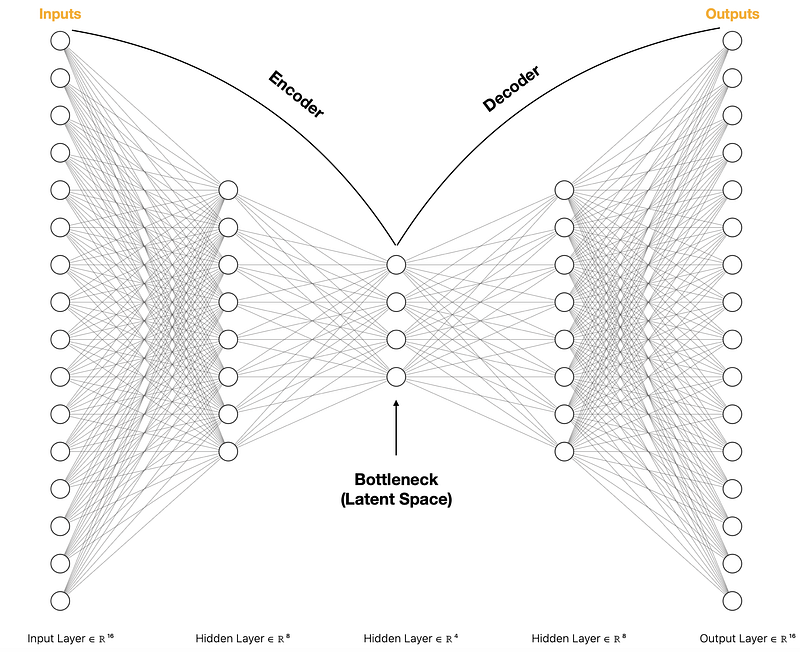
\includegraphics[width=0.7\textwidth]{figures/pic1_1.png}
	\caption{Пример структуры автоэнкодера [1]}
	\label{fig:pic1_1}
\end{figure}

Автоэнкодеры находят своё применение не только в задачах уменьшения размерности вектора, но и в задачах преобразования
исходных данных. Например, удаление шума с изображения, как показано на рисунке~\ref{fig:pic1_2}.

\begin{figure}[h!]
	\centering
	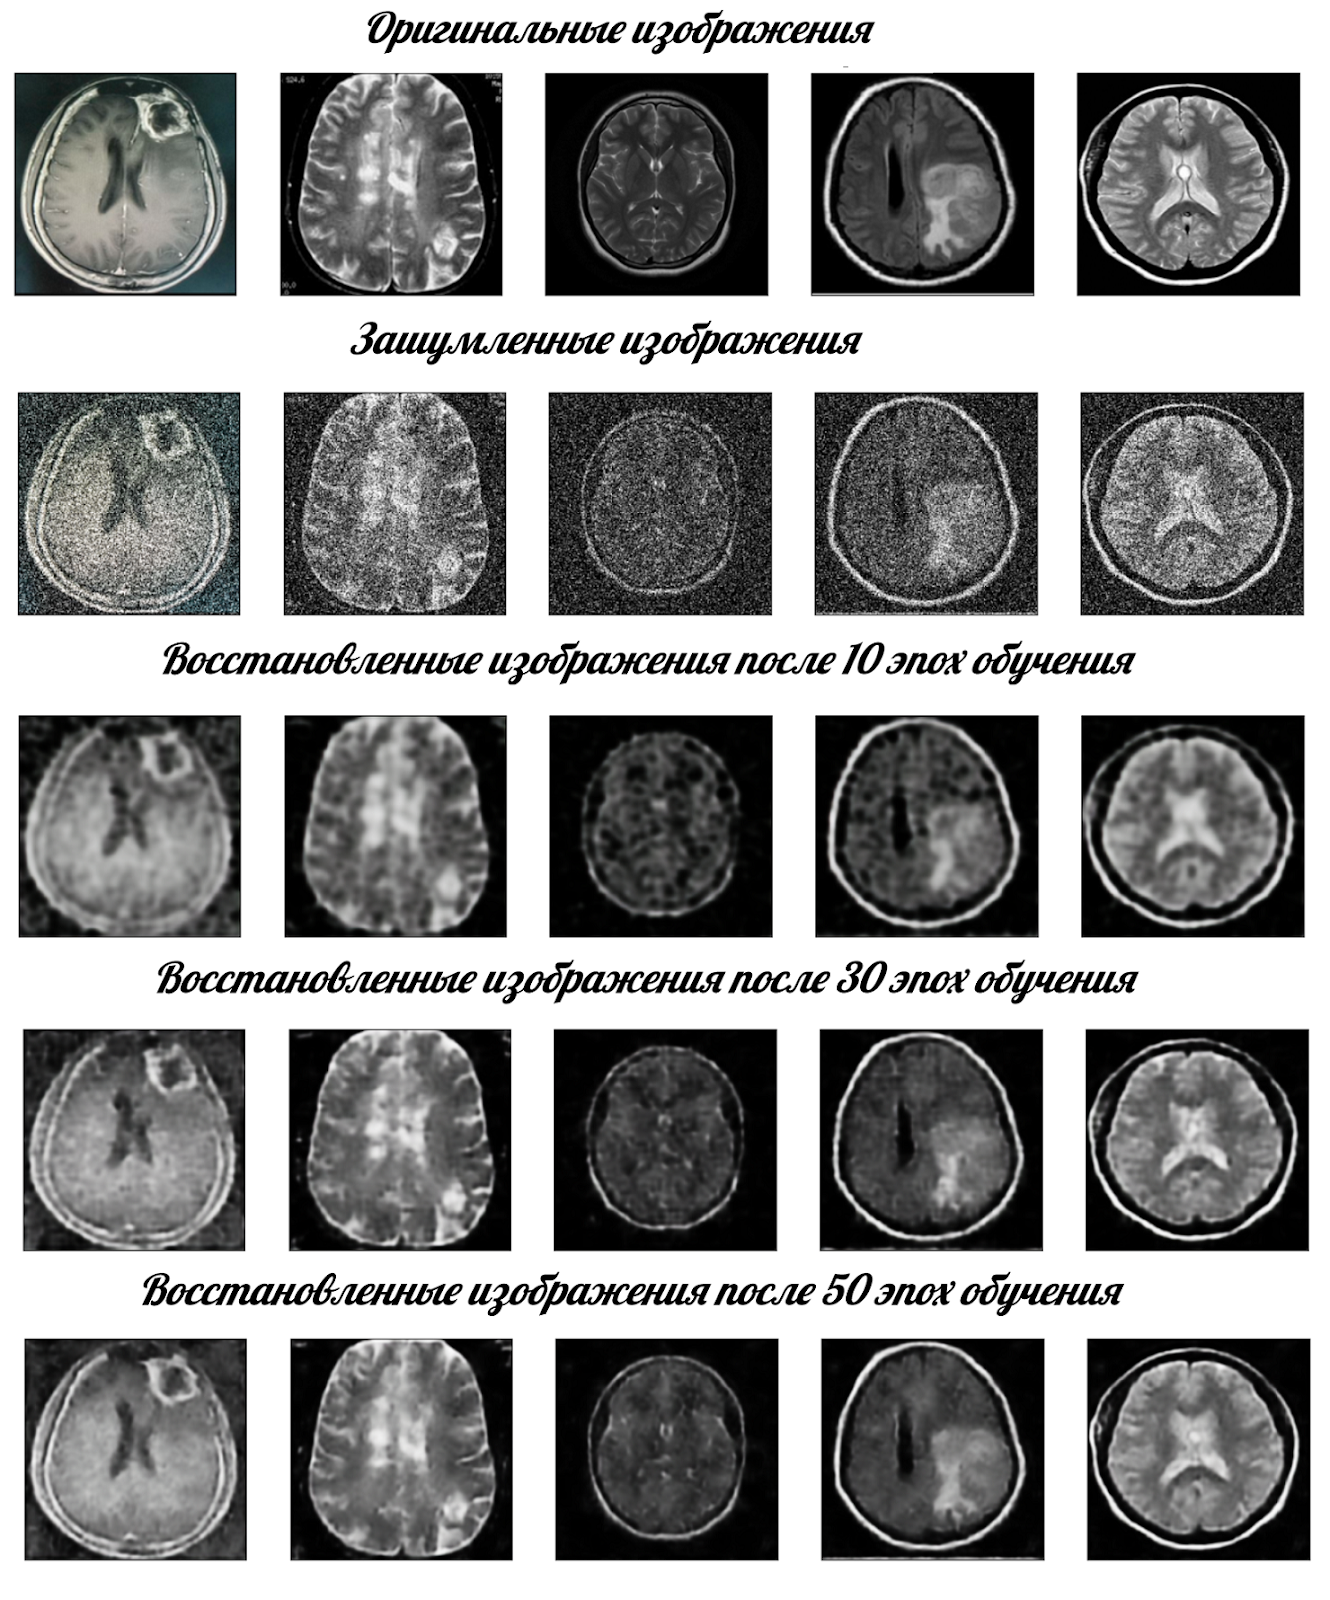
\includegraphics[width=0.6\textwidth]{figures/pic1_2.png}
	\caption{Удаление шума при помощи автоэнкодера [2]}
	\label{fig:pic1_2}
\end{figure}

У данной архитектуры нейронной сети для текущей задачи есть как положительные, так и отрицательные стороны. Часто для восстановления
музыкального отрезка очень важен контекст: что звучало до текущего отрезка, так как контекст содержит информацию о волнах. 
Некоторые особенно низкие частоты могут быть и не определены как частота в виду достаточно маленького времени. Минимально слышимая
для человеческого уха частота в ~20 Гц потребует около 0,05 секунд для проигрывания одного периода. Проблему контекста в данной
архитектуре можно решить при помощи увеличения фрейма, например, до 1 секунды. Этой информации будет достаточно для сохранения частот.
Однако с увеличением входного слоя увеличивается сложность обучения, требования к аппаратному обеспечению растут.

Есть и плюсы в использовании текущего подхода. Декодирование отдельных независящих друг от друга фреймов позволит масштабировать 
процесс декодирования при появлении более продвинутого аппаратного обеспечения путём параллельного декодирования. Кроме того, 
автоэнкодер довольно просто обучать и использовать.

\subsubsection{Обзор архитектуры перцептронов}

Как уже было сказано ранее, автоэнкодер может быть достаточно тяжёлой свёрточной нейросетью при использовании большого количества входных параметров.
Существуют способы оптимизации, позволяющие сократить количество связей между нейронами. 

\par\textbf{Полносвязная нейросеть}

Полносвязный слой строится по принципу "нейрон связан с каждым нейроном из предыдущего слоя". В контексте аудиоданных это может быть как
положительным примером, так и отрицательным. Так, например, более низкие частоты с большим периодом смогут влиять на значение текущего нейрона, 
а значит информация о низких частотах будет сохранена. Но полносвязные слои крайне неоптимизированны. Вместе с важными данными в нейрон
может приходить и "мусор", который будет только добавлять шума в декодированной записи. 

При использовании полносвязной нейросети требуется тонкая настройка входного слоя. Далеко не все данные могут быть полезными, и
слишком большой входной вектор может привести к очень большому времени достижения экстремума для нейронной сети при обучении.

\par\textbf{Использование Convolution слоёв}

Convolutional слои позволяют создавать неполносвязную нейронную сеть. На примере одномерного массива Conv-слой сможет выбирать лишь небольшой 
участок из более большого вектора. Кроме того, Convolution слои могут работать как с одномерными, так и с двумерными, трёхмерными слоями. 
Например, на рисунке~\ref{fig:pic1_3} изображён пример поведения Convolutional слоя. Он не использует при вычислении все
входные параметры, а выбирает только соответственно своему фильтру

\begin{figure}[h!]
	\centering
	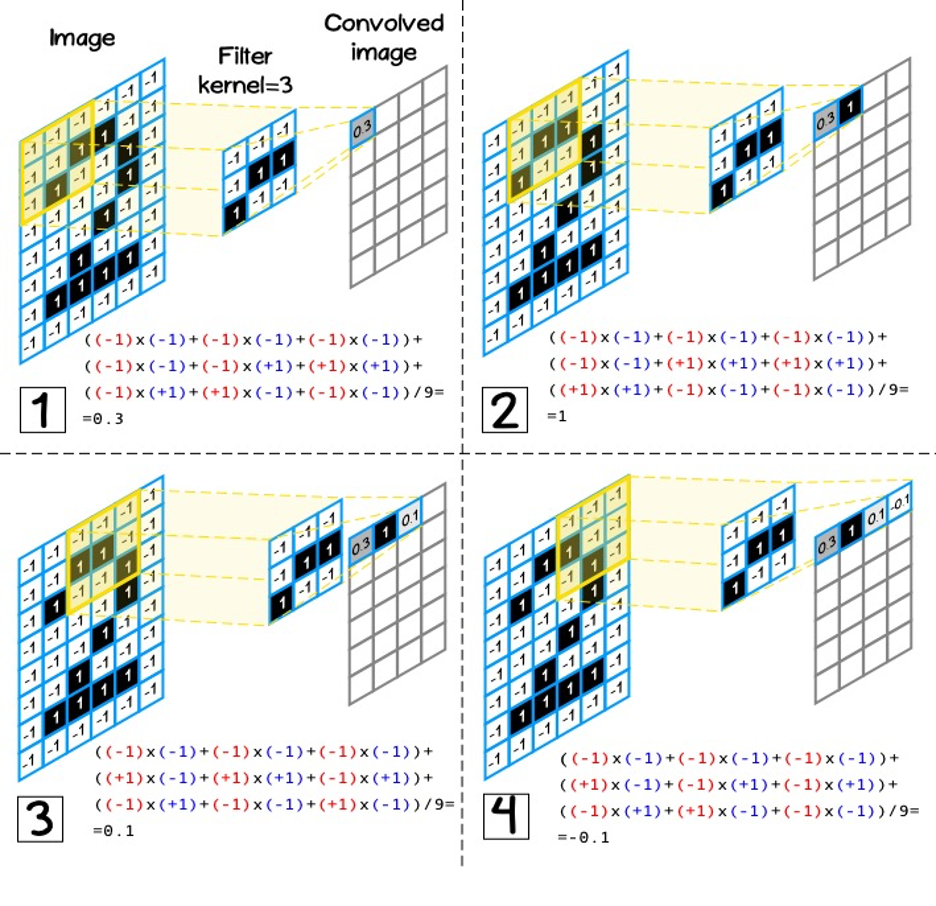
\includegraphics[width=0.7\textwidth]{figures/pic1_3.png}
	\caption{Принцип работы Convolutional Layer [3]}
	\label{fig:pic1_3}
\end{figure}

Использование Convolutional слоёв позволяет решить проблему слишком большой выборки данных, что позволит уменьшить количество связей
между нейронами. Уменьшение связей между нейронами позволит увеличить размер входного слоя, что позволит увеличить количество кодируемой/декодируемой
информации за один раз. Однако при использовании такого рода слоёв всё ещё остаётся проблема настройки выборки. Кроме того, при потоковой
распаковке аудио гораздо более ценна работа с относительно небольшим фреймом данных.

\subsubsection{Обзор преобразования входных данных}

Нейронные сети умеют работать с данными различных размерностей. Рассмотрим, в какие форматы данных можно было бы преобразовать аудиоданные. 

\par\textbf{Одномерный вектор}

Это самый простой способ. Аудиоданные преобразуются в одномерный массив, свойство каждого из которых содержит амплитуду. Этот способ относительно
лёгок в реализации и не требует больших преобразовательных мощностей, так как фактически выполняется преобразование аудиоданных в 
последовательность амплитуд, что естественно для большинства аудиоформатов на сегодняшний день, и производится дополнительная нормализация данных
для работы в нейронной сети.

\par\textbf{Двухмерная спектрограмма}

Можно преобразовать аудиоданные в более сложный и требующий больших вычислений формат. Спектрограмма представляет собой изображение. Одна из координат 
может представлять собой время, а другая - частоту. Яркость точки на изображении в точке (x, y) будет показывать, насколько сильна
амплитуда частоты x в момент y. Для получения такого изображения используются алгоритм быстрого преобразования Фурье. Для этого способа
так же требуется достаточно большой размер фрейма. Если фрейм будет недостаточно большим, то алгоритм просто "не услышит" длинные волны.
На рисунке~\ref{fig:pic1_4} представлена спектрограмма записи голоса человека, говорящего Hello World, после чего он кашляет. Видно
по первому всплеску, что у голоса есть определённый тон и повторяющиеся гребни - октавы. Кашель же - это в основном шум, поэтому основной тон там не так заметен.

\begin{figure}[h!]
	\centering
	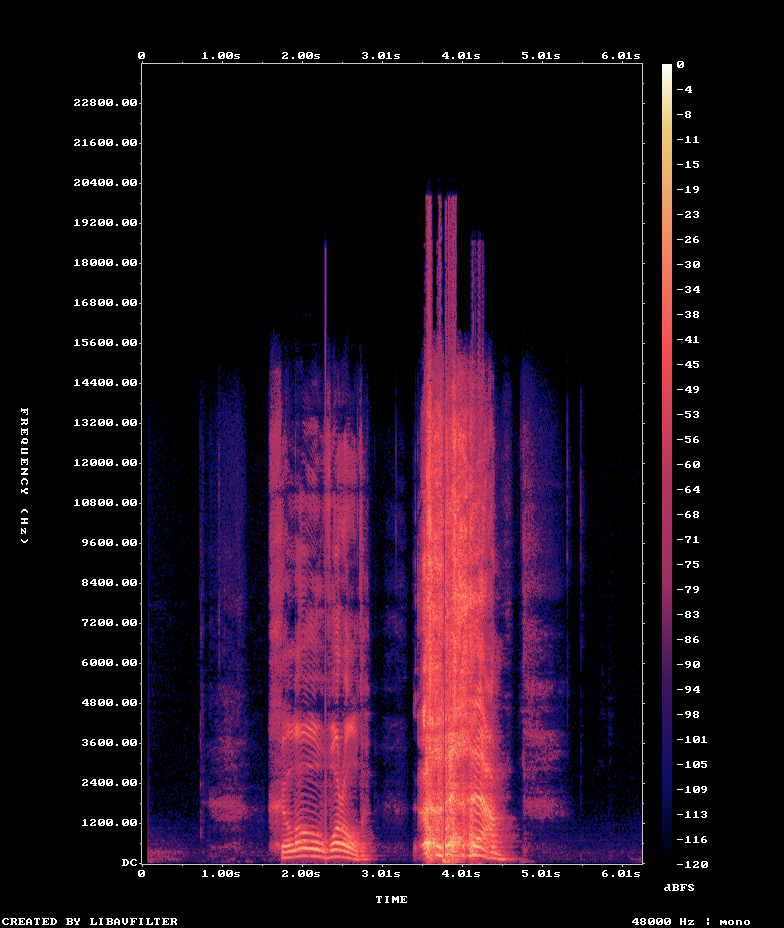
\includegraphics[width=0.6\textwidth]{figures/pic1_4.png}
	\caption{Запись голоса человека в спектрограмме, авторский материал}
	\label{fig:pic1_4}
\end{figure}

Использование такого подхода так же будет вызывать трудности и с декодированием спектрограммы. Для этого тоже используются специальные алгоритмы
Гриффина-Лима или обратного быстрого преобразования Фурье. Данный способ даёт большую нагрузку на аппаратное обеспечение и может вызывать задержки при
потоковой распаковке.

\subsubsection{Функции потерь}

Функции потери будут прямо влиять на процесс обучения и, соответственно, на получившееся звучание аудиоданных.
Именно функция потери определяет то, на что будет сфокусировано внимание при обучении.

\par\textbf{MSELoss}

Самая простая функция. Предположим, что у нас есть исходный сигнал $y$ и предсказанный сигнал $\overline{y}$ размерность $N$. Тогда функция потерь MSE будет высчитана как

$MSE = \frac{1}{N} \sum_{i=1}^{N}(y_i - \overline{y}_i) ^ 2$

Эта функция может быть не очень хороша для аудиоданных, так как она слабо учитывает отклонения во всплесках - в аудио это может быть
удар бочки или же по тарелке. Но она неплохо восстанавливает общую картинку и общую слышимость.

\par\textbf{Spectral Loss}

Функция спектральной потери считает потери по определённым частотам. Эта функция потери гораздо более близка к природе аудиоданных, 
так как работает с её частотами напрямую. Обычно высчитывается потеря по нескольким частотам отражающим одну ноту, например [128 Гц, 256 Гц, 512 Гц, 1024 Гц]. 
Для определения амплитуд частот используется быстрое преобразование Фурье.
Эта функция потерь гораздо лучше сохраняет детали, нежели общее звучание. Семейство функций спектральной потери часто используется при обучении
нейронных сетей, работающих с аудиоданными.

Положим, что у нас есть исходный сигнал $y$ и $\overline{y}$. Тогда функция спектральной потери будет высчитана следующим образом

$SpectralLoss = |log(|STFT(y)| + \epsilon) - log(|STFT(\overline{y})| + \epsilon)|$

Где $\epsilon$ - очень маленькая величина.

Чаще всего используется комбинированная функция потери в зависимости от цели при обучении.

\subsection{Постановка задачи}

На основе представленной информации можем сформировать список желаемого функционала в сервисе

\begin{itemize}
	\item Аутентификация и регистрация для управления бизнес сущностями.
	\item Возможность работы с авторами композиции.
	\begin{itemize}
		\item Автор должен содержать имя, аватар, описание
		\item Должны поддерживаться операции CRUD: добавление, удаление, редактирование и получение 
		\item Необходимо предоставить графический интерфейс для работы с указанными операциями
	\end{itemize}
	\item Возможность работы с группами
	\begin{itemize}
		\item Группа - это объединение авторов. Она должна включать в себя аватар, описание, участников
		\item Должны поддерживаться операции CRUD: добавление, удаление, редактирование и получение 
		\item Необходимо предоставить графический интерфейс для работы с указанными операциями
	\end{itemize}
	\item Возможность создавать песню
	\begin{itemize}
		\item Песня должна содержать в себе справочную информацию: имя, описание, тэг, BPM, тональность, слова, авторов и группы а также файлы этой песни.
		\item Должна быть возможность указать ведущих файлов. Эти файлы репрезентируют песню. Так, ведущее изображение является картинкой этой песни. А ведущее аудио - проигрывающей песней при её запуске. Дополнительные файлы могут содержать прочую важную информацию.
		\item После создания песню удалить нельзя - можно только выпустить следующий релиз песни. Всегда можно просмотреть предыдущие релизы песен.
		\item Должен быть доступен чат внутри каждой из песен, где пользователи могут просматривать а также отправлять свои собственные сообщения
		\item Должна быть реализована возможность просмотра конкретной версии песни.
		\item Должны быть реализованы операции в API для выполнения вышеобозначенных операций.
		\item Необходимо предоставить графический интерфейс для работы с указанными операциями.
	\end{itemize}
	\item Плейлист
	\begin{itemize}
		\item Плейлист - это сущность, которая собирает в себе песни и фильтрует их по фильтру. Плейлист должен в себя включать изображение, название и описание.
		\item Функция фильтрации заключается в поиске по текстовому полю, который может представлять собой либо название тега либо название версии. Если указано название тега, в песне должна быть найдена наиболее новая песня с указанным тегом. Если фильтр не указан, будет предоставлена последняя версия песни. Если же указан номер версии, будет найдена версия с этим конкретным номером.
		\item Должны быть реализованы операции CRUD: добавление, удаление, редактирование и получение
		\item Должен быть предоставлен графический интерфейс для взаимодействия с указанными операциями.
	\end{itemize}
	\item Взаимодействие с файлами
	\begin{itemize}
		\item Должен быть предоставлен альтернативный способ хранения аудиоданных, использующий доверенный кодек для хранения аудиоданных.
		\item Необходимо предоставить возможность скачивать загруженные файлы
		\item Отправка аудиоданных со своим кодеком должна поддерживать специальные заголовки, позволяющие получать данные порционно. Распаковка не должна происходить одномоментно и должна распаковываться постепенно.
	\end{itemize}
	\item Проигрыватель
	\begin{itemize}
		\item Должен быть реализован проигрыватель, позволяющий проиграть плейлист или же отдельную версию песни.
		\item Плейлист должен поддерживать следующие операции: выбрать порядок в пределах плейлиста (перемешать, в обычном порядке, зациклить), выбрать порядок в передлах песни (зациклить песню или разрешить переход к следующим), выбрать следующий трек, выбрать предыдущий трек, отразить информацию о песне, выбрать громкость.
		\item Должно быть реализовано API достаточное для выполнения описанных функций
		\item Должен быть реализован графический интерфейс, поддерживающий эти операции
	\end{itemize}
	
\end{itemize}


\end{document}